%%%%%%%%%%%%%%%%%%%%%%%%%%%%%%%%%%%%%%%%%%%%%%%%%%%%%%%%%%%
\subsection{Statistical model design and testing}
%%%%%%%%%%%%%%%%%%%%%%%%%%%%%%%%%%%%%%%%%%%%%%%%%%%%%%%%%%%
%
%
\begin{frame}[t, negative]
	\subsectionpage
\end{frame}
%
%
\begin{lhframe}[rhgraphic={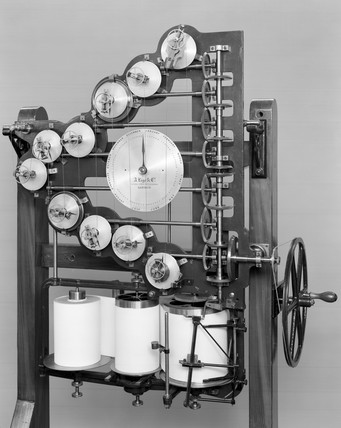
\includegraphics[scale=2]{tide_machine.jpg}}]
	{Model design and test\footnote{Following \citet{Fogarty_et_al_2022}}}
	
	Purpose:
	%
	\begin{itemize}
		%
		\item to have reliable procedures,
		\item to maintain a clear documentation,
		\item to have a sound analysis
		%
	\end{itemize}
	
	Procedure:
	%
	\begin{itemize}
		%
		\item step by step, instantiating one difficulty at the time
		%
		\item use probabilistic assumptions defined in \textcolor{blue}{estimand and process model}
		%
		\item is like running \textcolor{blue}{synthetic data generation} backwards
		%
	\end{itemize}
	%
\end{lhframe}
%
%
\begin{lhframe}[rhgraphic={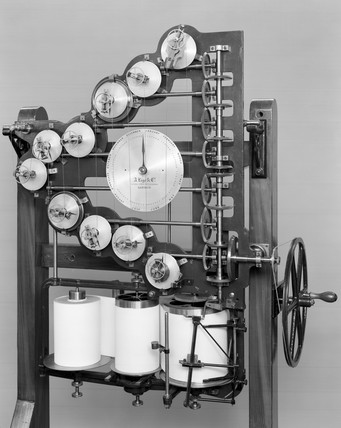
\includegraphics[scale=2]{tide_machine.jpg}}]
	{Model design and test}
	
	We evaluate,
	%
	\begin{itemize}
		%
		\item the probabilistic model implementation \cite{McElreath_2020, Betancourt_et_al_2013} \\
		{\small (centered and non-centered versions) }
		%
		\item prior predictive
		\item ``health" of MCMC chains
		\item parameter recovery
		\item posterior predictive
		\item power
		%
	\end{itemize}
	% 
\end{lhframe}
%
%
\begin{lhframe}[rhgraphic={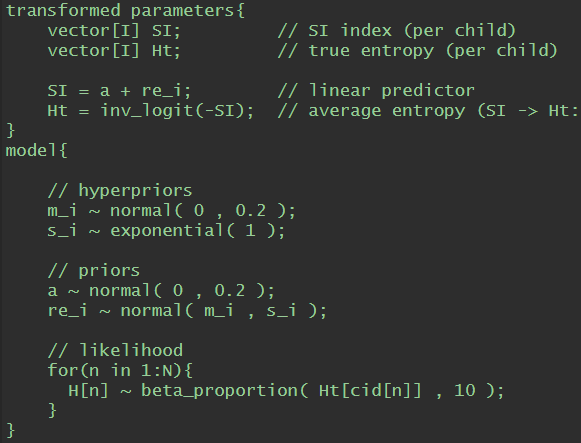
\includegraphics[scale=0.59]{model_design1.png}}]
	{Probabilistic model}
	
	starts with,
	%
	\begin{itemize}
		%
		\item the simplest model
		\item the simplest data generating procedure
		%
	\end{itemize}
	% 
\end{lhframe}
%
%
\begin{lhframe}[rhgraphic={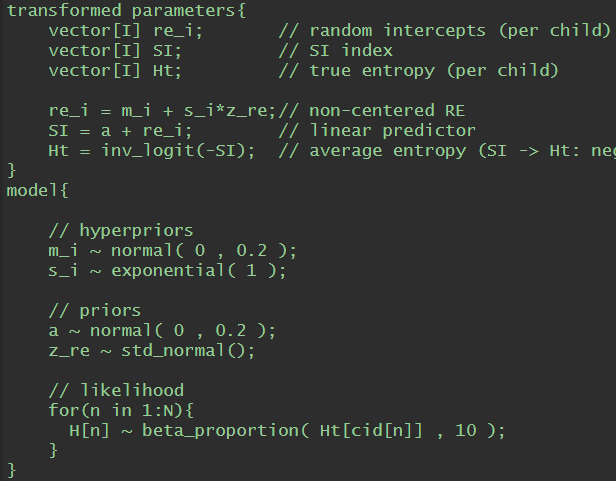
\includegraphics[scale=0.59]{model_design2.png}}]
	{Probabilistic model}
	
	try,
	%
	\begin{itemize}
		%
		\item the centered and non-centered parametrization
		%
	\end{itemize}
	% 
\end{lhframe}
%
%
\begin{lhframe}[rhgraphic={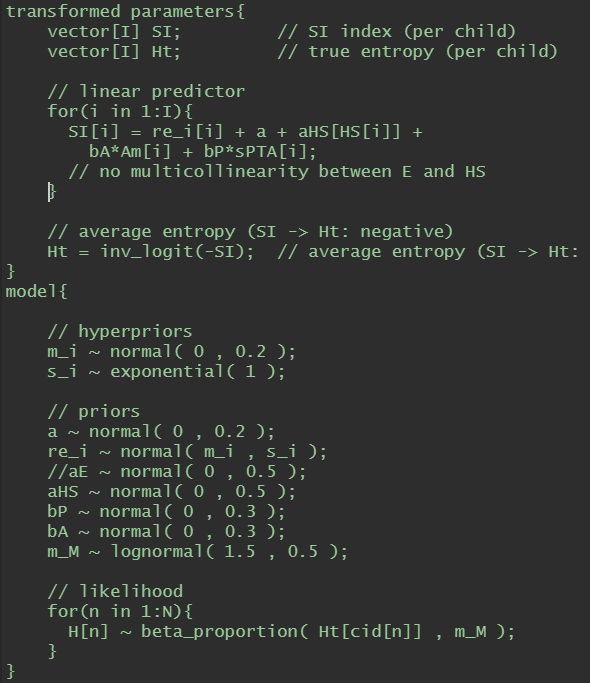
\includegraphics[scale=0.59]{model_design3.png}}]
	{Probabilistic model}
	
	escalate,
	%
	\begin{itemize}
		%
		\item complexity of model
		\item traits of the data
		%
	\end{itemize}
	%
\end{lhframe}
%
%
\begin{lhframe}[rhgraphic={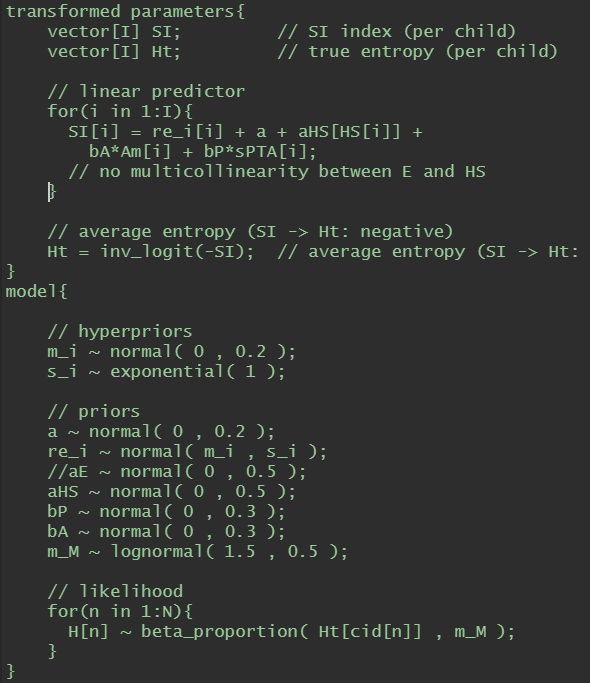
\includegraphics[scale=0.55]{model_design3.png}}]
	{Probabilistic model}
	
	We tested $5$ random effects models: \\
	{\small (from $5$ synthetic data types)} \\ 
	{\small (centered, and non-centered)}
	%
	\begin{itemize}
		%
		\item only intercept, $M=10$, 
		%
		\item causal model, $M=10$,
		%
		\item causal model, $M$ per individual,
		%
		\item no known process,
		%
		\item causal model with interactions, \\
		$M$ per individual,
		%
	\end{itemize}
	%
\end{lhframe}
%
%
\begin{frame}
	{Prior predictive}
	%
	\begin{columns}
		%
		\begin{column}{0.5\textwidth}
			%
			Priors and hyper-priors
			%
			\begin{itemize}
				%
				\item In the \textcolor{blue}{probabilistic (causal) model} there were no priors for our parameters,
				%
				\item To decide our priors we follow \citet{McElreath_2020}: \\ \textcolor{blue}{``priors are part of the assumptions, and should be inspected as such"},
				%
				\item We will evaluate the implications of our priors on the outcome scale. \\
				We have \textcolor{blue}{three outcomes scales}: \\
				$SI_{i}$, $H^{T}_{i}$, and $H^{O}_{ik}$
				%
			\end{itemize}
			%
		\end{column}
		%
		\begin{column}{0.5\textwidth}  
			%
			\begin{equ}
				%
				\begin{aligned} 
					%
					\text{Priors}\\
					a_{i} & \sim \; Normal( \mu_{a}, \sigma_{a}) \\
					M_{i} & \sim \; LogNormal( \mu_{M}, \sigma_{M}) \\
					\alpha & \sim \; Normal( 0, 0.2) \\
					\alpha_{HS[i]} & \sim \; Normal( 0, 0.3) \\
					\alpha_{E[i]} & \sim \; Normal( 0, 0.3) \\ 
					\beta_{A, HS[i]} & \sim \; Normal( 0, 0.3) \\
					\beta_{P} & \sim \; Normal( 0, 0.3) \\
					%
					\text{Hyper-priors} \\
					\mu_{a} & \sim \; Normal( 0, 0.2) \\
					\sigma_{a} & \sim \; Exp(1) \\
					\mu_{M} & \sim \; Normal( 0, 0.5) \\
					\sigma_{M} & \sim \; Exp(1) \\
					%
				\end{aligned}
				%
			\end{equ}
			%
		\end{column}
		%
	\end{columns}
	%
\end{frame}
%
%
\begin{lhframe}[rhgraphic={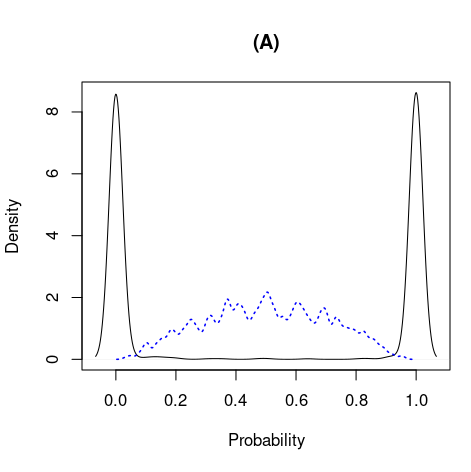
\includegraphics[scale=0.5]{prior_elicitation.png}}]
	{Prior predictive}
	
	Undesired assumptions can easily creep in \textcolor{blue}{non-linear models}\footnote{Figure extracted from \citet{Rivera_2021}.} \\
	Example:
	%
	\begin{align*}
		\text{ \small{(\textcolor{black}{black} line)} } & \\
		\theta & \sim N(0,100) \\
		logit(p) & =  \theta
	\end{align*}
	%
	\begin{align*}
		\text{ \small{(\textcolor{blue}{blue} line)} } & \\
		\theta & \sim N(0,1) \\
		logit(p) & =  \theta
	\end{align*}
	%
\end{lhframe}
%
%
\begin{lhframe}[rhgraphic={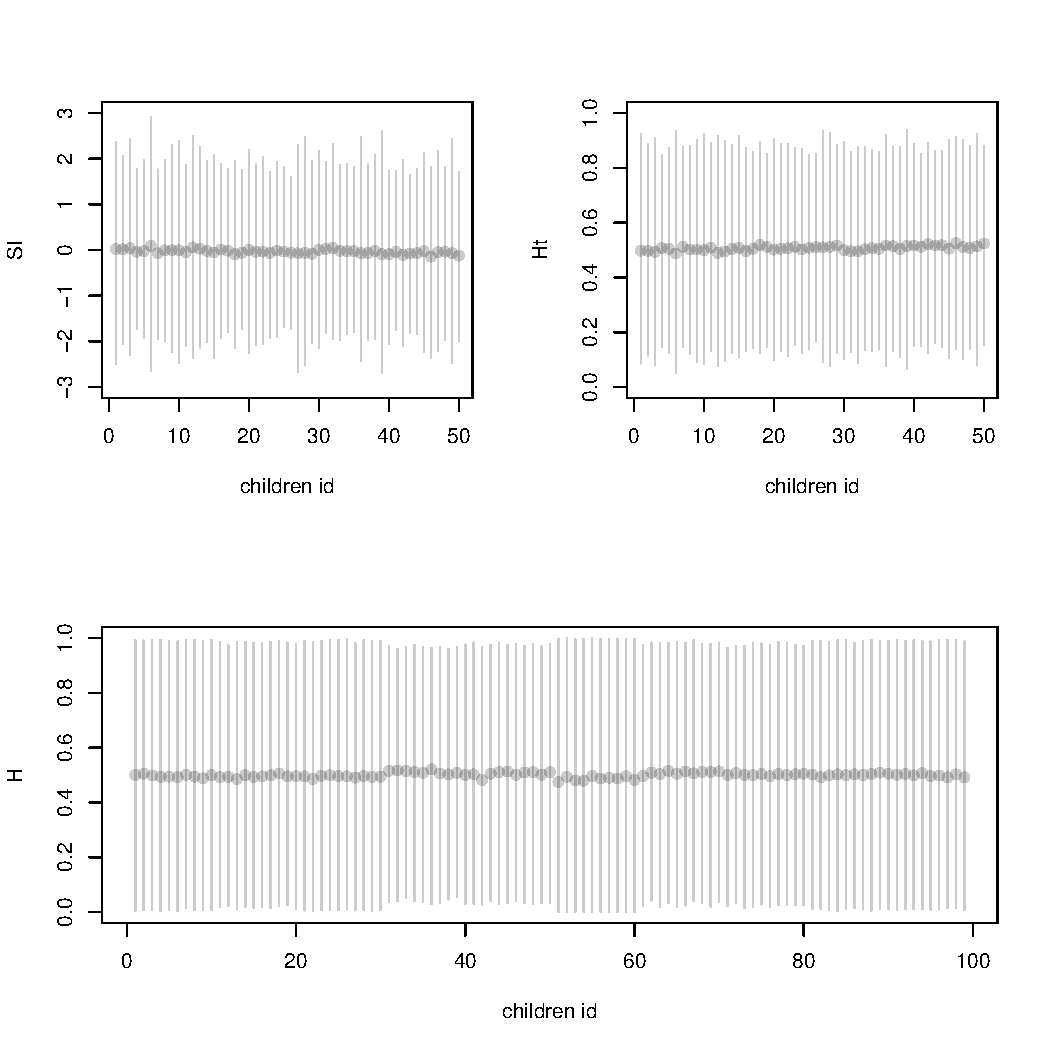
\includegraphics[scale=0.43]{prior_predictive.pdf}}]
	{Prior predictive}
	
	What our priors imply? \\ \\
	\textcolor{blue}{NO undesired assumption} has crept in:
	\begin{itemize}
		%
		\item the $SI_{i}$ scale,
		\item the $H^{T}_{i}$ scale,
		\item the $H^{O}_{ik}$ scale
		%
	\end{itemize}
	
	i.e. the \textcolor{blue}{scales' full space can be reached} by (a combination of) the parameters
	%
\end{lhframe}
%
%
\begin{lhframe}[rhgraphic={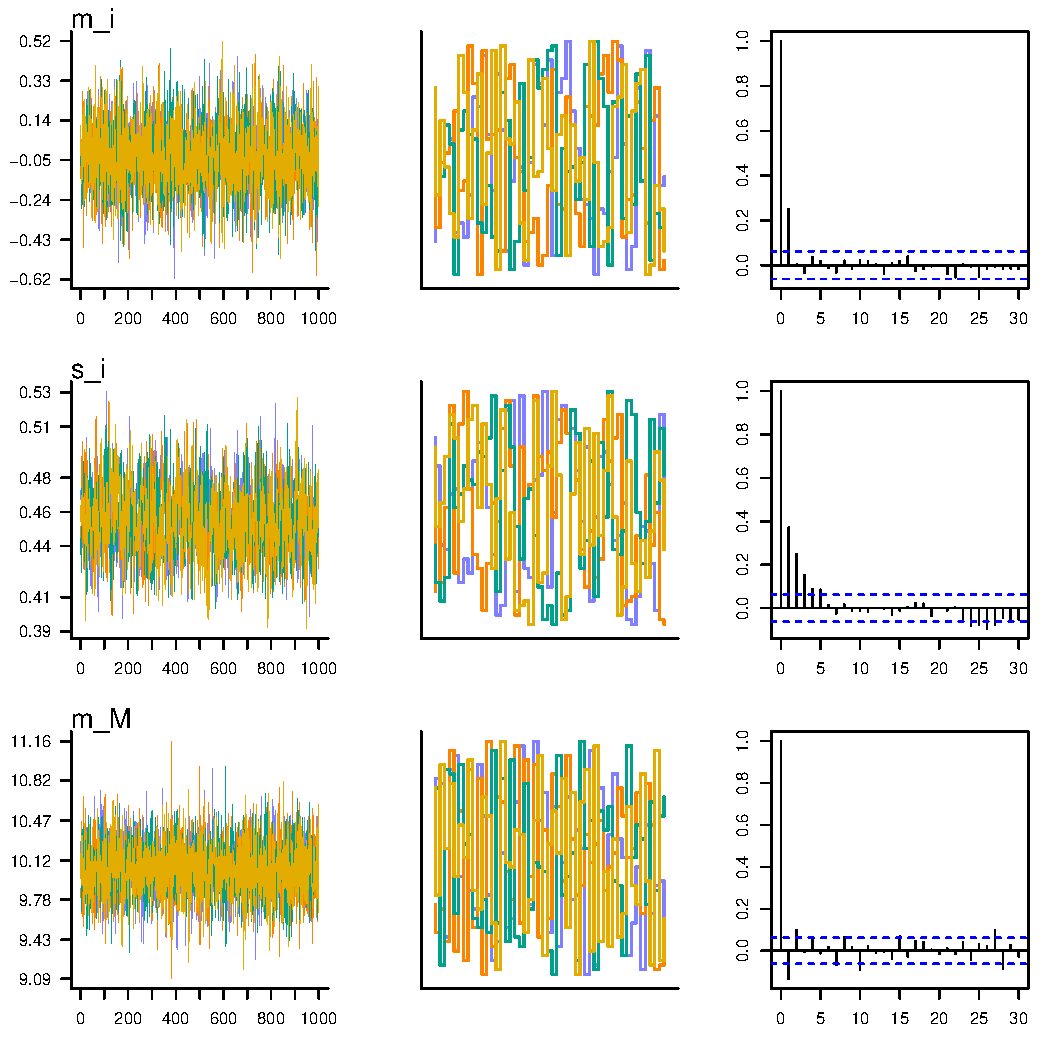
\includegraphics[scale=0.40]{chains1.pdf}}]
	{``Health" of MCMC chains}
	
	The MCMC chains achieve,
	%
	\begin{itemize}
		%
		\item good convergence
		\item good mixing
		\item lack of autocorrelation
		%
	\end{itemize}
	
	same results on the \textcolor{blue}{ \texttt{n\_eff} } and \textcolor{blue}{ \texttt{RHat} } statistics.
	%
\end{lhframe}
%
%
\begin{lhframe}[rhgraphic={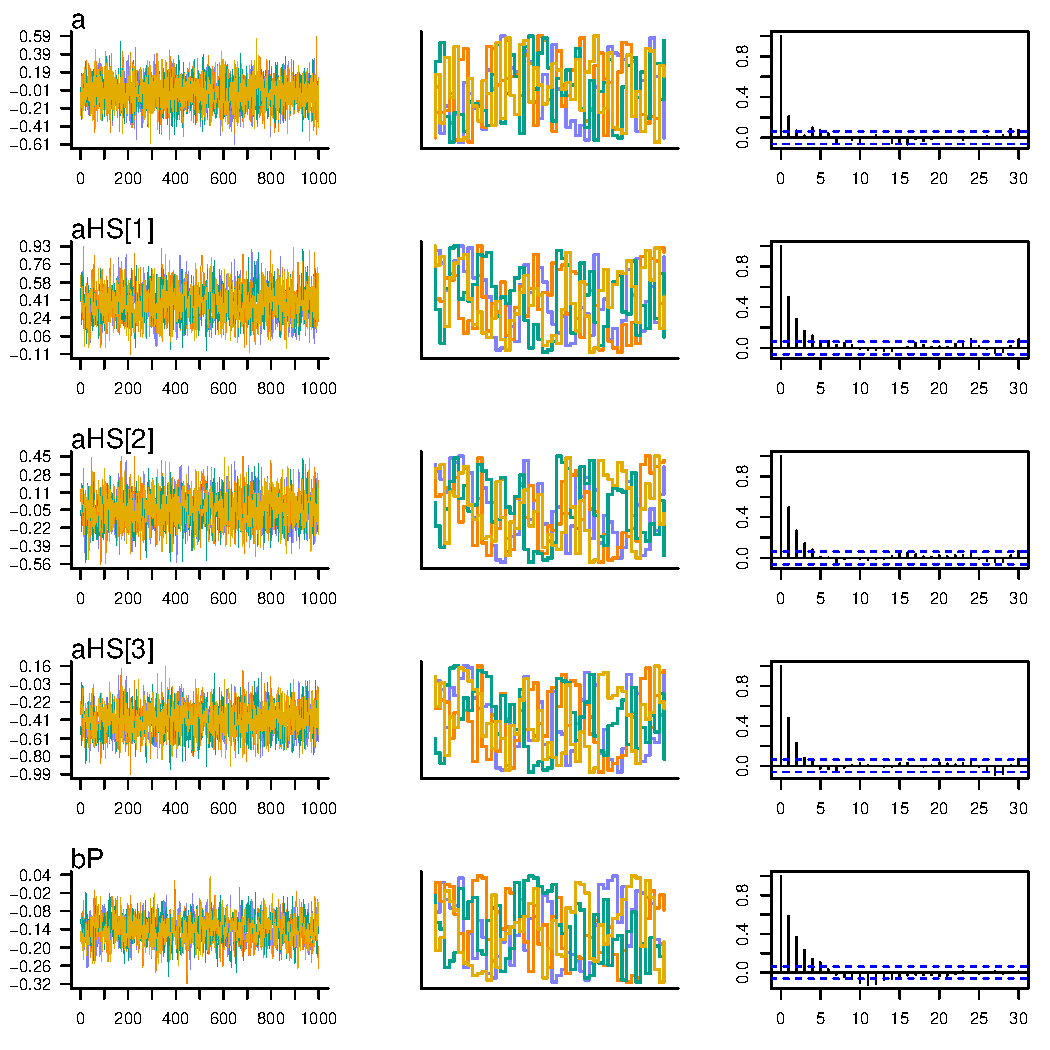
\includegraphics[scale=0.40]{chains2.pdf}}]
	{``Health" of MCMC chains}
	
	The MCMC chains achieve,
	%
	\begin{itemize}
		%
		\item good convergence
		\item good mixing
		\item lack of autocorrelation
		%
	\end{itemize}
	
	same results on the \textcolor{blue}{ \texttt{n\_eff} } and \textcolor{blue}{ \texttt{RHat} } statistics.
	%
\end{lhframe}
%
%
\begin{lhframe}[rhgraphic={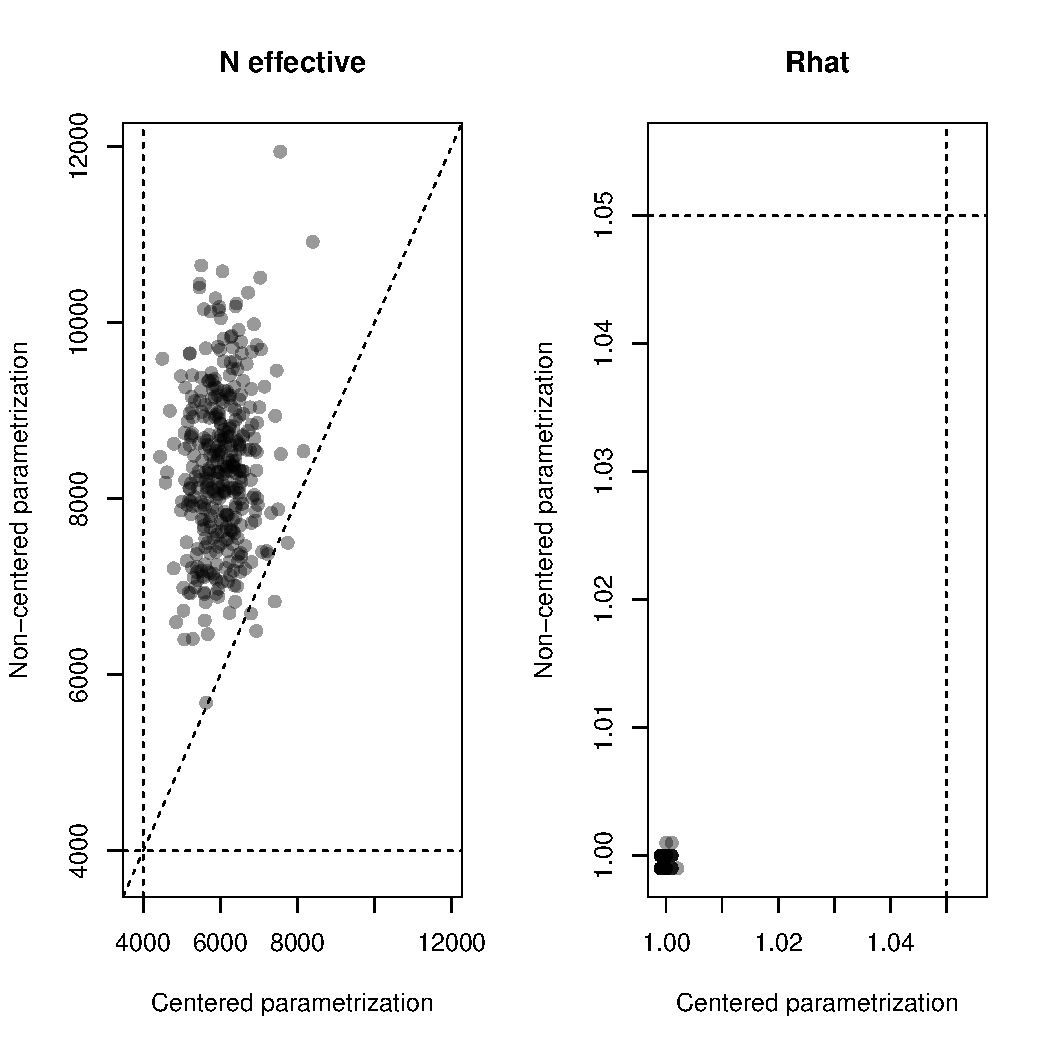
\includegraphics[scale=0.38]{chain_stat.pdf}}]
	{``Health" of MCMC chains}
	
	The non-centered parametrization has,
	%
	\begin{itemize}
		%
		\item better \textcolor{blue}{ \texttt{n\_eff} } \\
		(denoting lack of autocorrelation)
		\item better \textcolor{blue}{ \texttt{Rhat} } \\
		(denoting good convergence)
		\item better mixing \\
		(inspected visually, not shown)
		%
	\end{itemize}
	%
\end{lhframe}
%
%
\begin{lhframe}[rhgraphic={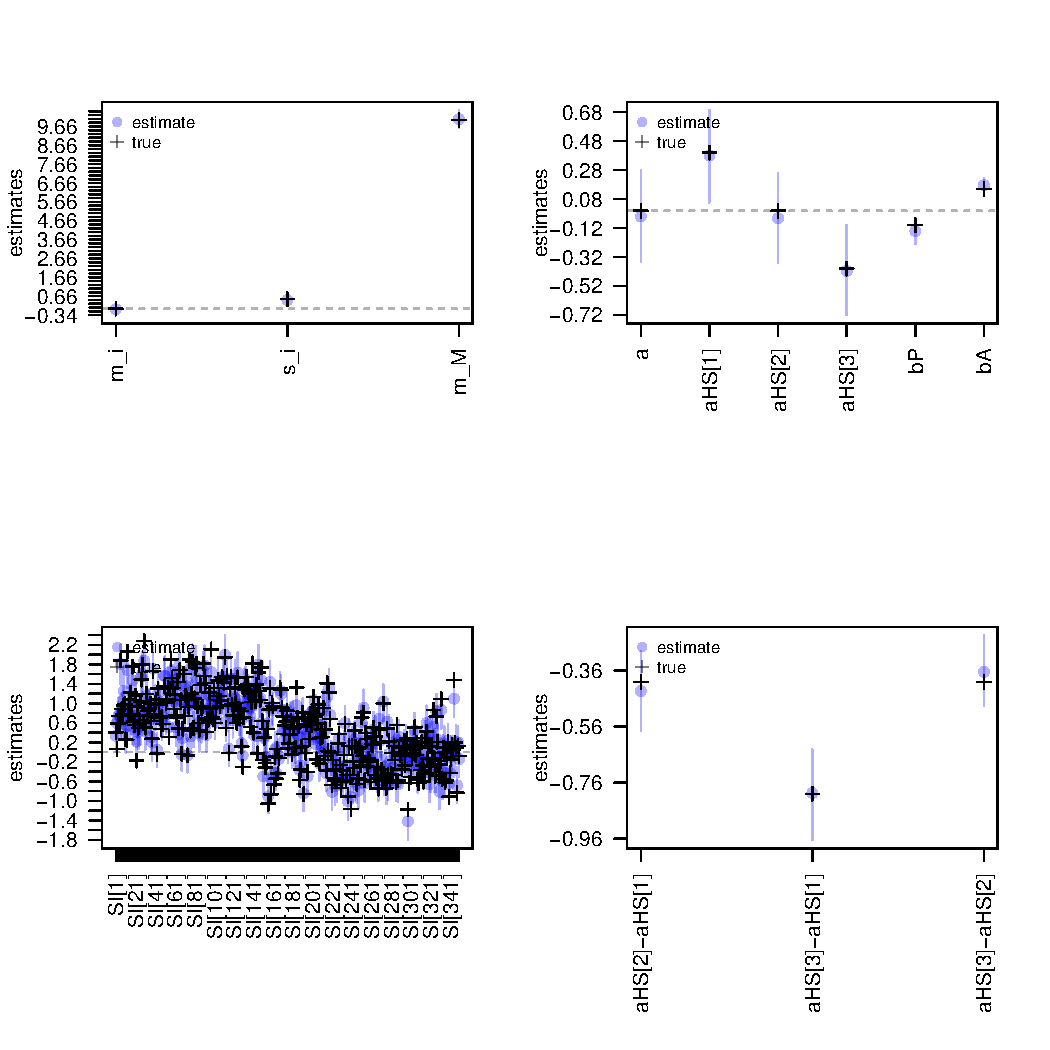
\includegraphics[scale=0.37]{recovery.pdf}}]
	{Parameter recovery}
	{On idealized data}
	
	The model,
	\subheading{with \textcolor{blue}{less working assumptions}\footnote{random effects causal model, with $M=10$}}
	%
	\begin{itemize}
		%
		\item recovers the parameters in the right scale,
		\item most of the ``true" parameters are inside of the \textcolor{blue}{compatibility intervals (CI)}
		\item contrast are approximately correct
		%
	\end{itemize}
	%
\end{lhframe}
%
%
\begin{lhframe}[rhgraphic={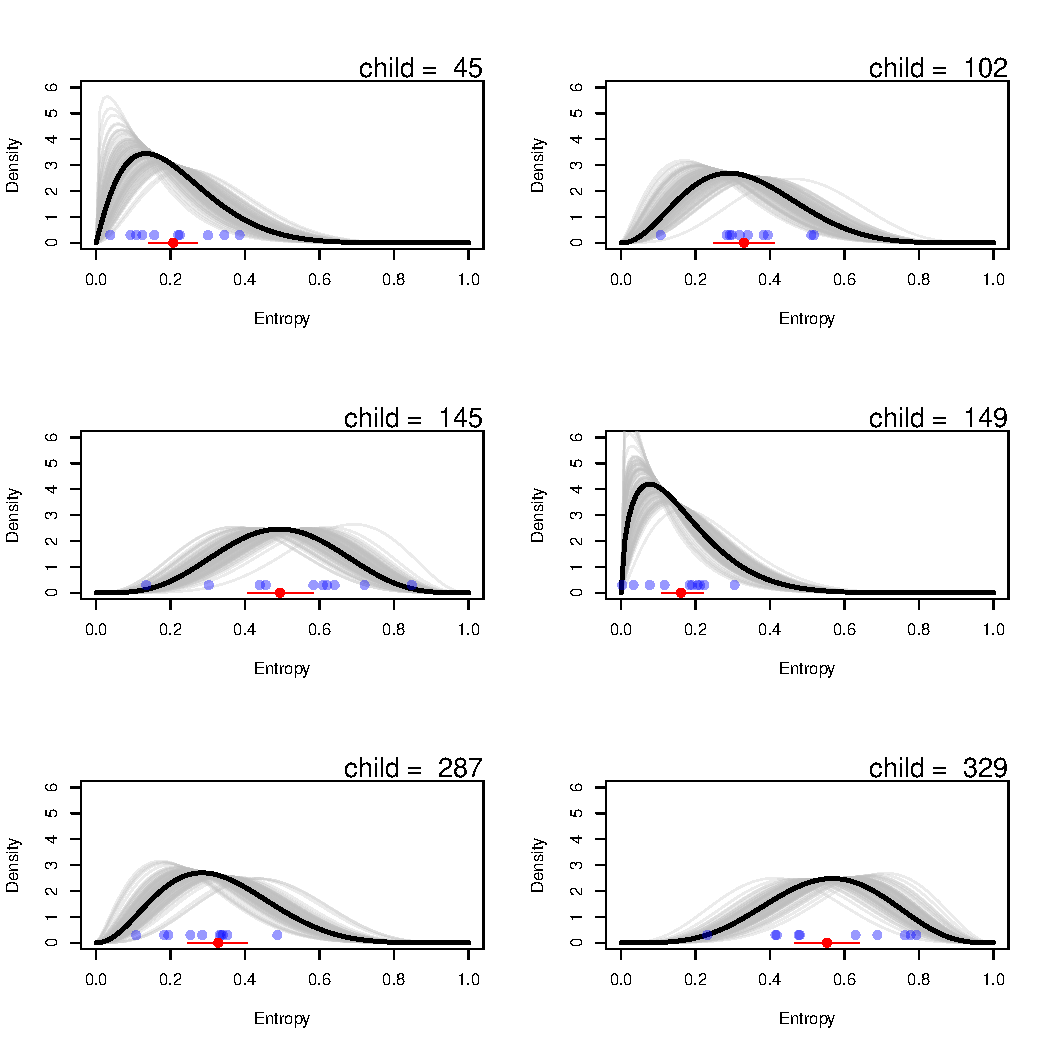
\includegraphics[scale=0.36]{posterior_predictive.pdf}}]
	{Posterior predictive}
	
	But how well reproduces the data?,
	\subheading{with \textcolor{blue}{less working assumptions}\footnote{random effects causal model, with $M=10$}}
	%
	\begin{itemize}
		%
		\item captures the variability of the replicates,
		\item provides a ``true" $H$ and $SI$
		%
	\end{itemize}
	
	More complex models, 
	\begin{itemize}
		%
		\item captures even better the data, but might \textcolor{blue}{overfit},
		\item avoid \textcolor{blue}{overfit} when the model is fit to the data (ITA \cite{Anderson_2008, Chamberlain_1965})
		%
	\end{itemize}
	%
\end{lhframe}
%
%
\begin{frame}
	{Power}
	{Equivalent prior sampling method \cite{Winkler_1967, Kruschke_2014}} 
	
	\begin{figure}
		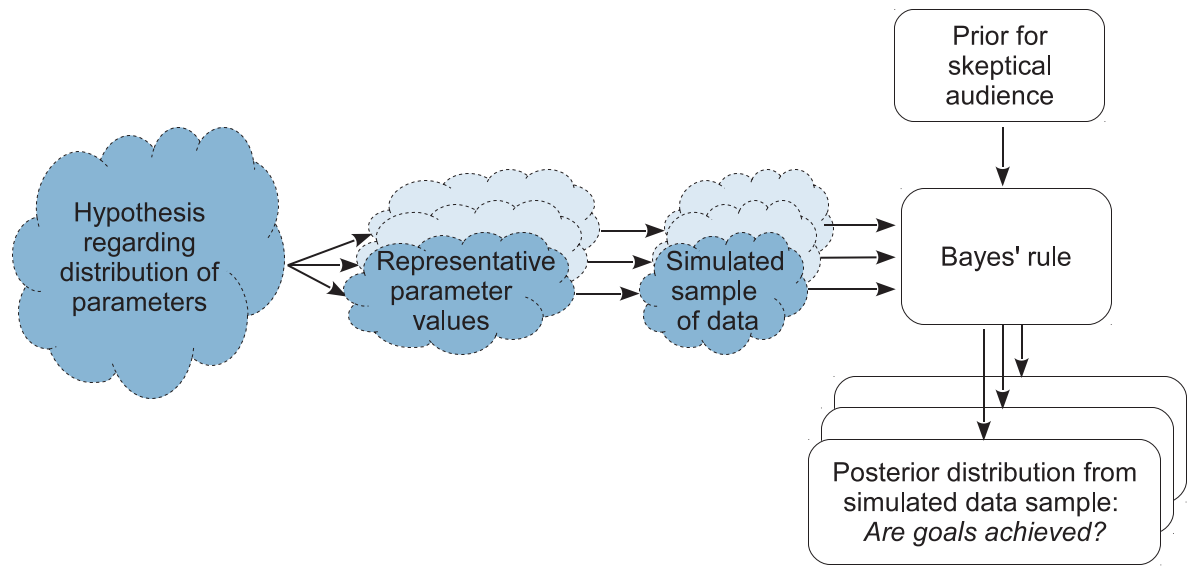
\includegraphics[scale=0.45]{power_process.png}
		\caption{ Flow of information in a power analysis, in which simulated data come from random hypothetical parameters. Extracted from \citet{Kruschke_2014}. }
	\end{figure}
	%
\end{frame}
%
%
\begin{lhframe}[rhgraphic={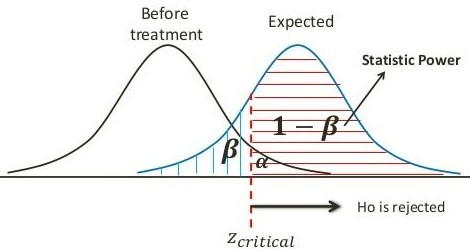
\includegraphics[scale=0.55]{power_image.jpg}}]
	{Power}
	{Equivalent prior sampling method} 
	%
	\begin{enumerate}
		%
		\item generate idealized data 
		%
		\item generate parameters' distribution \\
		\small{(with Bayes theorem)}
		%
		\item simulate data sample \\
		\small{ (variability in data and parameters) }
		%
		\item apply models to simulated data \\
		\small{ (include priors) }
		%
		\item evaluate desire goals
		%
		\begin{itemize}
			\item reject the null hypothesis
			\item affirm predicted value
			\item achieve precision in estimate
		\end{itemize}
		%
		\item repeat procedure \\
		\small{ (to approximate power) }
		%
	\end{enumerate}
	%
\end{lhframe}
%
%
\begin{lhframe}[rhgraphic={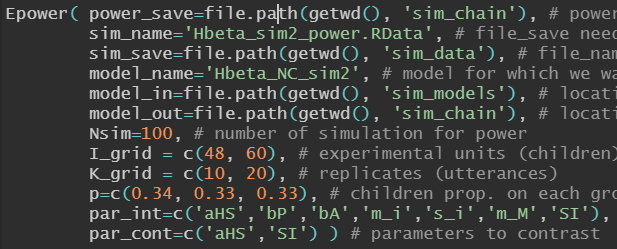
\includegraphics[scale=0.50]{power_function.png}}]
	{Power}
	{Equivalent prior sampling method} 
	%
	\begin{enumerate}
		%
		\item \sout{generate idealized data}
		%
		\item \sout{generate parameters' distribution} \\
		\small{(with Bayes theorem)}
		%
		\item \textcolor{blue}{simulate data sample} \\
		\small{ (variability in data and parameters) }
		%
		\item \textcolor{blue}{apply models to simulated data} \\
		\small{ (include priors) }
		%
		\item evaluate desire goals
		%
		\begin{itemize}
			\item reject the null hypothesis
			\item affirm predicted value
			\item achieve precision in estimate
		\end{itemize}
		%
		\item repeat procedure \\
		\small{ (to approximate power) }
		%
	\end{enumerate}
	%
\end{lhframe}
%
%
\begin{lhframe}[rhgraphic={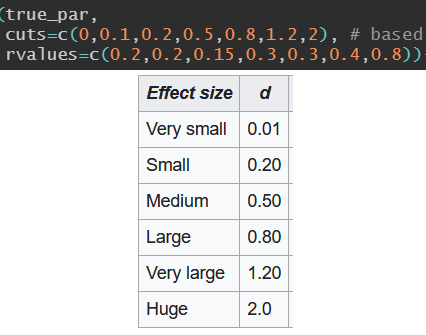
\includegraphics[scale=0.40]{ES_ROPE.png}}]
	{Power}
	{Equivalent prior sampling method} 
	%
	\begin{enumerate}
		%
		\item \sout{generate idealized data}
		%
		\item \sout{generate parameters' distribution} \\
		\small{(with Bayes theorem)}
		%
		\item \sout{simulate data sample} \\
		\small{(variability in data and parameters)}
		%
		\item \sout{apply models to simulated data} \\
		\small{(include priors)}
		%
		\item \textcolor{blue}{evaluate desire goals}\footnote{use ROPE \cite{Kruschke_2014}, and effect sizes \cite{Cohen_1988, Sawilowsky_2009}}
		%
		\begin{itemize}
			\item reject the null hypothesis
			\item affirm predicted value
			\item achieve precision in estimate
		\end{itemize}
		%
		\item \textcolor{blue}{repeat procedure} \\
		\small{ (to approximate power) }
		%
	\end{enumerate}
	%
\end{lhframe}
%
%
\begin{lhframe}[rhgraphic={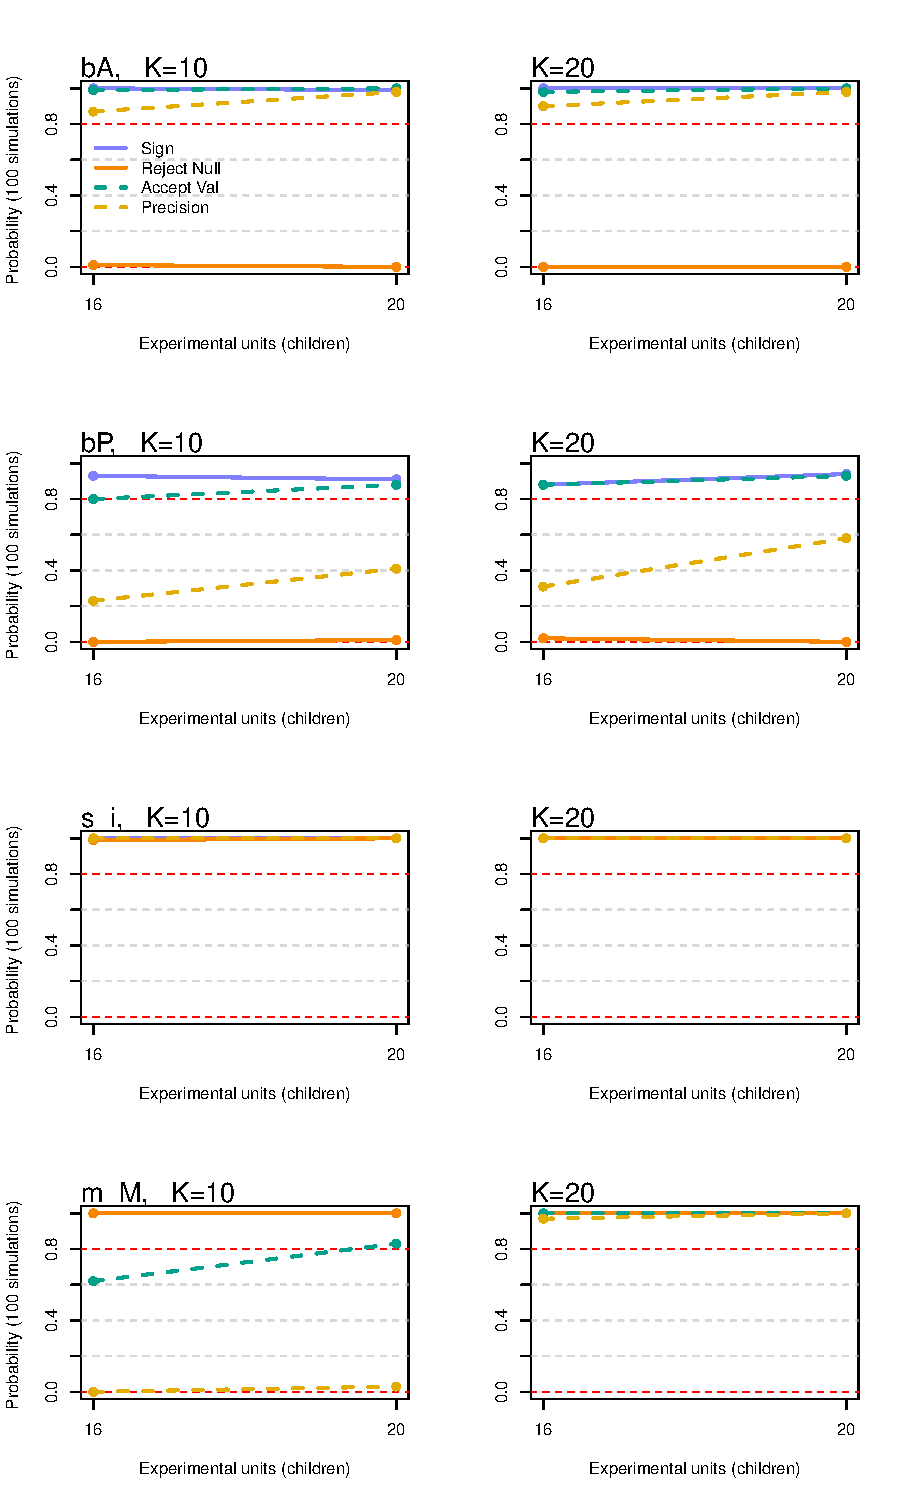
\includegraphics[scale=0.35]{power_result1.pdf}}]
	{Power results} 
	
	For this parameter set,
	%
	\begin{itemize}
		%
		\item reject the null hypothesis, \\
		never achieved in \textcolor{blue}{structural parameters},
		%
		\item affirm predicted value, \\
		in \textcolor{blue}{all} shown parameters
		%
		\item achieve precision in estimate, \\
		in \textcolor{blue}{some} parameters is reached
		%
	\end{itemize}
	
	Notice,
	%
	\begin{itemize}
		%
		\item between child $SI$ variability,
		\item replicates measurement error ($M$),
		\item not much difference with $2x$ comparisons {\small(except for $M$)}
		%
	\end{itemize}
	%
\end{lhframe}
%
%
\begin{lhframe}[rhgraphic={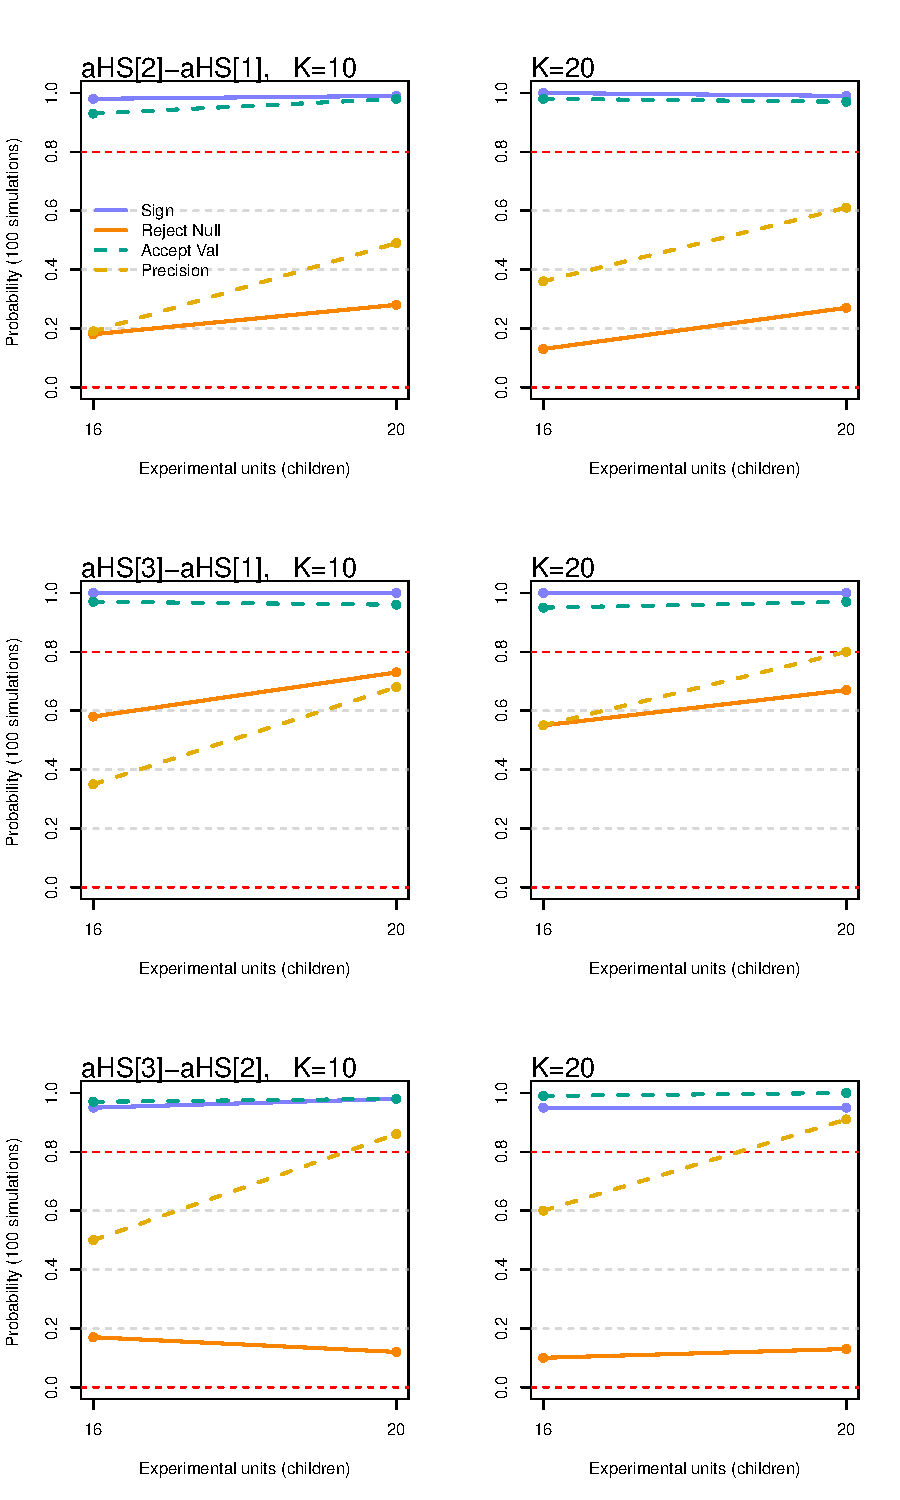
\includegraphics[scale=0.35]{power_result2.pdf}}]
	{Power results} 
	
	For group contrasts,
	%
	\begin{itemize}
		%
		\item reject the null hypothesis, \\
		closest for the \textcolor{blue}{largest contrast},
		%
		\item affirm predicted value, \\
		in \textcolor{blue}{all} shown contrasts,
		%
		\item achieve precision in estimate, \\
		\textcolor{blue}{grows} with more children
		%
	\end{itemize}
	
	Notice,
	%
	\begin{itemize}
		%
		\item not much difference with $2x$ comparisons
		\item group contrasts are easier to identify {\small (larger sample size per comparison) }
		%
	\end{itemize}
	%
\end{lhframe}
%
%
\begin{lhframe}[rhgraphic={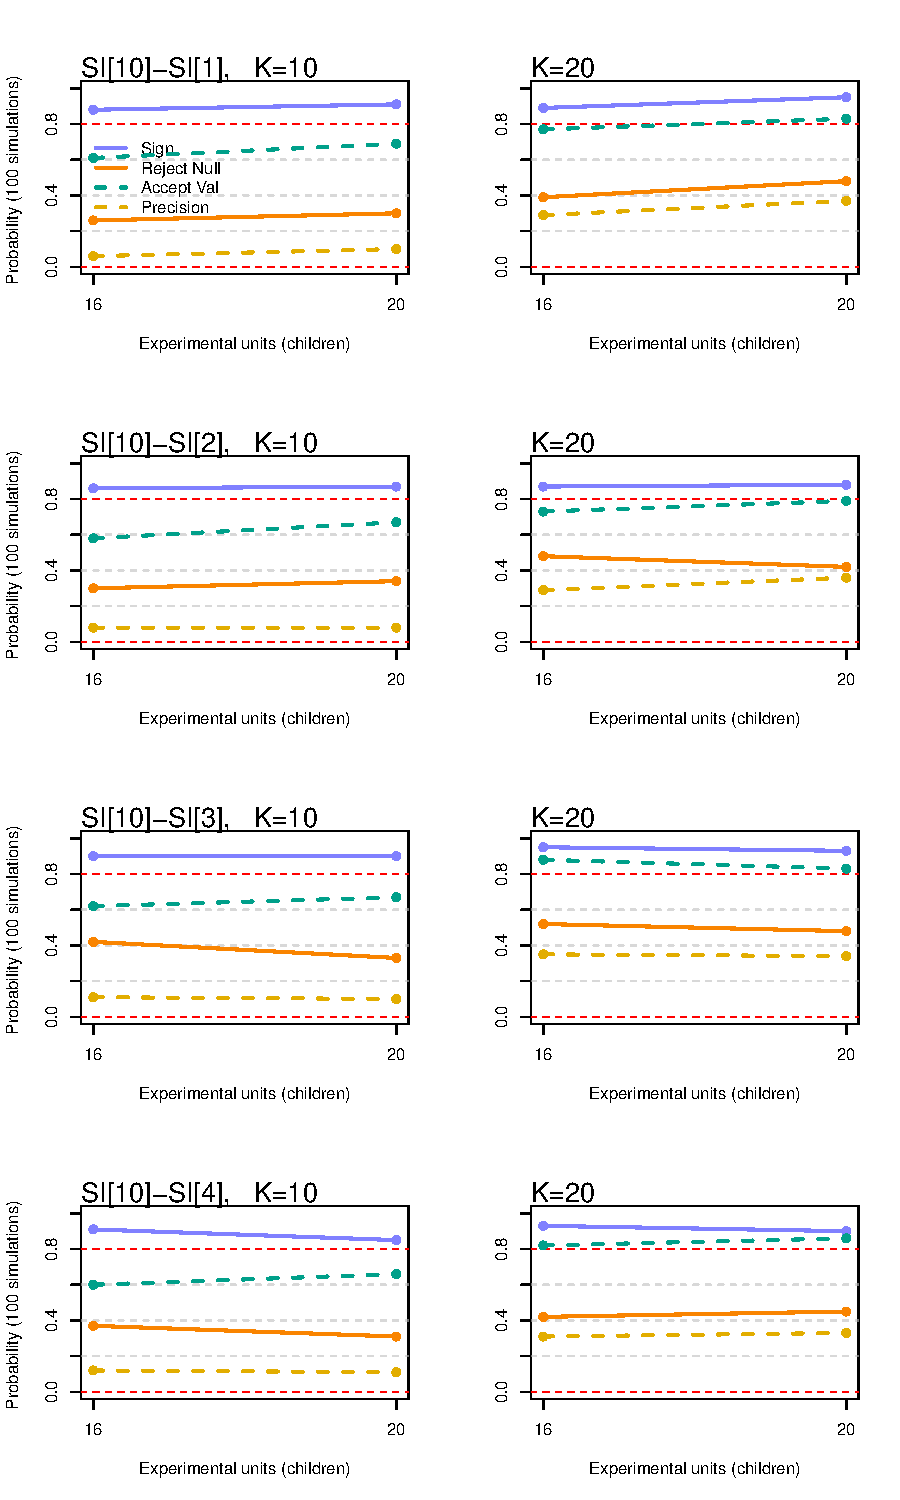
\includegraphics[scale=0.35]{power_result3.pdf}}]
	{Power results} 
	
	For individual contrasts,
	%
	\begin{itemize}
		%
		\item reject the null hypothesis, \\
		\textcolor{blue}{depends} on the contrast of interest,
		%
		\item affirm predicted value, \\
		for \textcolor{blue}{some} is achieved,
		%
		\item achieve precision in estimate, \\
		clearly requires more sample size
		%
	\end{itemize}
	
	Notice,
	%
	\begin{itemize}
		%
		\item we see a clear difference with $2x$ comparisons {\small (more sample at the appropriate level) }
		%
	\end{itemize}
	%
\end{lhframe}
%
%
